\chapter{Experiments} \label{chap:experiments}

In this section, we will introduce the experiment we are conducting and showcase different steps we are undertaking to conduct our experiment, among a few other things. After that, we will list our clear goals, hypothesis and expectations from the experiment, as well as our hardware and software environment configuration. Then, we will set up and start conducting the experiment while simultaneously explaining and justifying each steps during the process.

After the experiment, we will first collect the data produced. We will then start analysing and categorising the collected data, process them and present them in the "Result" section. Furthermore, we will provide our verdict of the experiment by delivering discussions on the investigation itself, such as whether the result was mainly within our expectations or perhaps the results differ from our initial assumption and prediction by a considerable margin.

Finally, we will list the challenges we faced, the irregularities we found during our experiment, and possible future work that might be worth undertaking in the "Discussion" section.

\bigskip
\section{WebAssembly framework options}

Our experiment will focus on the two categories of microservice frameworks: \textbf{VM/Container-Based frameworks} and \textbf{WebAssembly-Based frameworks}. In addition, with each experiment scenario, we will run it in our local environment as well as on the cloud computing services.

Here are some of the WebAssembly frameworks we are interested in. In this section, we will compare and analyse and, in addition, identify the \textbf{strengths}, \textbf{weaknesses} as well as \textbf{characteristics} of each of the frameworks. Ultimately, we will choose a framework that aligns most with our interests.

\bigskip
\begin{table}[h!]
\centering
\begin{tabular}{||c c c||} 
\hline
Name & Developer & Website \\ [1ex] 
\hline\hline
 & & \\
Sledge & George Washington University & github.com/gwsystems/sledge-serverless-framework \\ 
 & & \\
Spin & Fermyon & github.com/fermyon/spin \\
 & & \\
WasmEdge (Runtime) & Linux foundation & wasmedge.org \\
 & & \\
Krustlet (Kubelet) & Deislabs & krustlet.dev \\
 & & \\
WAGI & Deislabs & github.com/deislabs/wagi \\
 & & \\
Wasmcloud & Wasmcloud team & wasmcloud.dev \\ [1ex]
\hline
\end{tabular}
\caption{List of WebAssembly frameworks of interest}
\label{table:webassembly_frameworks}
\end{table}

\bigskip
\subsection{Sledge}

The Sledge framework was created and developed by researchers at \textbf{George Washington University}. It offers a fast yet lightweight user experience, and it is designed to be run using WebAssembly runtimes natively. On top of that, the researchers have also developed a custom WASM runtime for it, called \textbf{AWSM} \cite{exp32} (pronounced Awesome), using the \textbf{Rust language} \cite{exp33}. However, both projects have yet to be production ready and are still in the testing phase. Adding on to that, they have yet to provide official deployment instructions for the framework.

\bigskip
\subsection{Spin}

The Spin framework by the Fermyon company is one of the most popular server-side WebAssembly frameworks out there at the moment. It is also featured in multiple news articles, including \textbf{Yahoo! Finance} \cite{exp34} and \textbf{Forbes} \cite{exp35}. Although not fully production ready yet, a considerable amount of testing has been done on the framework, and it has gained significant attention within the server-side backend community.

On top of that, Fermyon has implemented and documented a detailed set of deployment instructions for Spin. In addition, they created their own Platform-as-a-service solution - \textbf{Fermyon cloud}, to host and manage Fermyon applications. They also teamed up with \textbf{Deislabs}, another major company in the WebAssembly server-side market, to deploy spin applications to \textbf{Amazon Web Service} through its \textbf{Hippo} bundler.

\bigskip
\subsection{WAGI}

WAGI is a product made by the aforementioned \textbf{Deislabs}. It is a super lightweight WebAssembly HTTP framework in its very early stage of development. WAGI is just like Spin in many ways. It is able to compile the code down to WASM32-WASI, which is a type of WebAssembly binary code. Therefore, it can run with any programming languages that compile to WASM32-WASI, such as Rust and Go. However, unlike Spin, it is only classified as experimental code, and Deislabs currently does not have the plan to further develop WAGI into a production-ready product. It also does not have an official deployment method.

\bigskip
\subsection{Wasmcloud}

Wasmcloud is a server-side backend framework and runtime that runs on all three major operating systems, Windows, macOS and Linux. On top of that, it is a polyglot platform that allows the same application to be developed using multiple programming languages. In this case, \textbf{AssemblyScript}, \textbf{Go} or \textbf{Rust}. It was designed with security and scalability in mind. It also functions as an ecosystem where each function is called an "actor", Wasmcloud provides its own Paas cloud computing service to deploy server-side applications, IoT applications, and client-side applications running in web browsers. Furthermore, it has built-in edge support and detailed instructions and documentation on the deployment procedure.

\bigskip
\section{Decision on Frameworks and Environment}

We start by choosing a WebAssembly framework. We looked at the properties of the WebAssembly frameworks above, and we decided to go with \textbf{Spin by Fermyon}. A few reasons contributes to this decision. First, Spin has a very detailed set of documentation, as well as example projects. More crucially, there is a research gap here as there have yet to be any tests performed on Spin running on the edge.

On the other hand, the other non-WebAssembly traditional framework we will be utilising in our experiment is \textbf{Flask} \cite{exp19}. As stated above, Flask is a Python HTTP microservice framework. It is currently one of the most famous traditional non-Webassembly frameworks, and Python is also one of the most popular programming languages.

The local environment for conducting our experiments will be on a \textbf{2017 MacBook Pro} running with the Intel Core I5-7267U CPU (2 cores, 3.1 GHz). It has 8GB memory with 512GB internal SSD storage. We will use \textbf{Amazon Web Service} for our cloud and edge deployment for the production environment. Specifically, we will utilise the \textbf{Amazon EC2} service to host our applications \cite{exp36}. Amazon EC2 offers a wide range of instances (server computers) that suit most businesses' needs, ranging from small IoT controller computers to large industrial servers for server farms \cite{exp37}. In our case, both of our frameworks will be deployed and run on an \textbf{AWS t3} micro instance. The t3 micro instance is a medium rage server. It has 2 vCPUs (Intel Xeon or AMD EPYC, both running up to 3.1 GHz) with 1GB memory and on-demand elastic storage (it charges its customers based on the amount of storage it holds). It is designed to run applications such as microservices, small to medium databases, business-critical applications and so on \cite{exp38}. It is small yet agile enough to be used as an edge server for our Spin application, but also powerful enough to host our Flask application for it to run in a traditional cloud environment.

\bigskip
\section{Roadblocks in Early Stage of Experiment}

The initial experiment plan is very distinct from the procedure described in this section. In the early stage of carrying out the experiment, we planned to integrate \textbf{PolyBench/C} into our benchmarking experiment \cite{exp39}. PolyBench is one of the best system benchmarking frameworks at the moment, and it is originally written in \textbf{C} and the \textbf{Fortran} language by \textbf{Louis-Noel Pouchet} at The \textbf{Ohio State University} \cite{exp40}. At first, we looked into benchmarking both of our frameworks with \textbf{PolyBench/Python} \cite{exp41}. This is a reimplementation of the original PolyBench/C and it was developed by Abella-Gonzalez et al. at the University of A Coruna in Spain alongside Louis-Noel Pouchet himself. However, when browsing through the project code, we discovered that PolyBench/Python is only available for x86 architecture machines running with Linux due to a number of runtime dependencies only available on the Linux operating system. Initially, we did not have access to such devices, but we later installed a copy of Ubuntu Linux operating system as a virtual machine through Oracle VM VirtualBox \cite{exp42} \cite{exp43}. However, in the end, we decided we won't go ahead with PolyBench/Python due to the potential system compatibility issues we might have on deployment. Therefore, we continued our experiment with the original PolyBench/C framework.

\bigskip
\begin{figure}[hp]
\centering
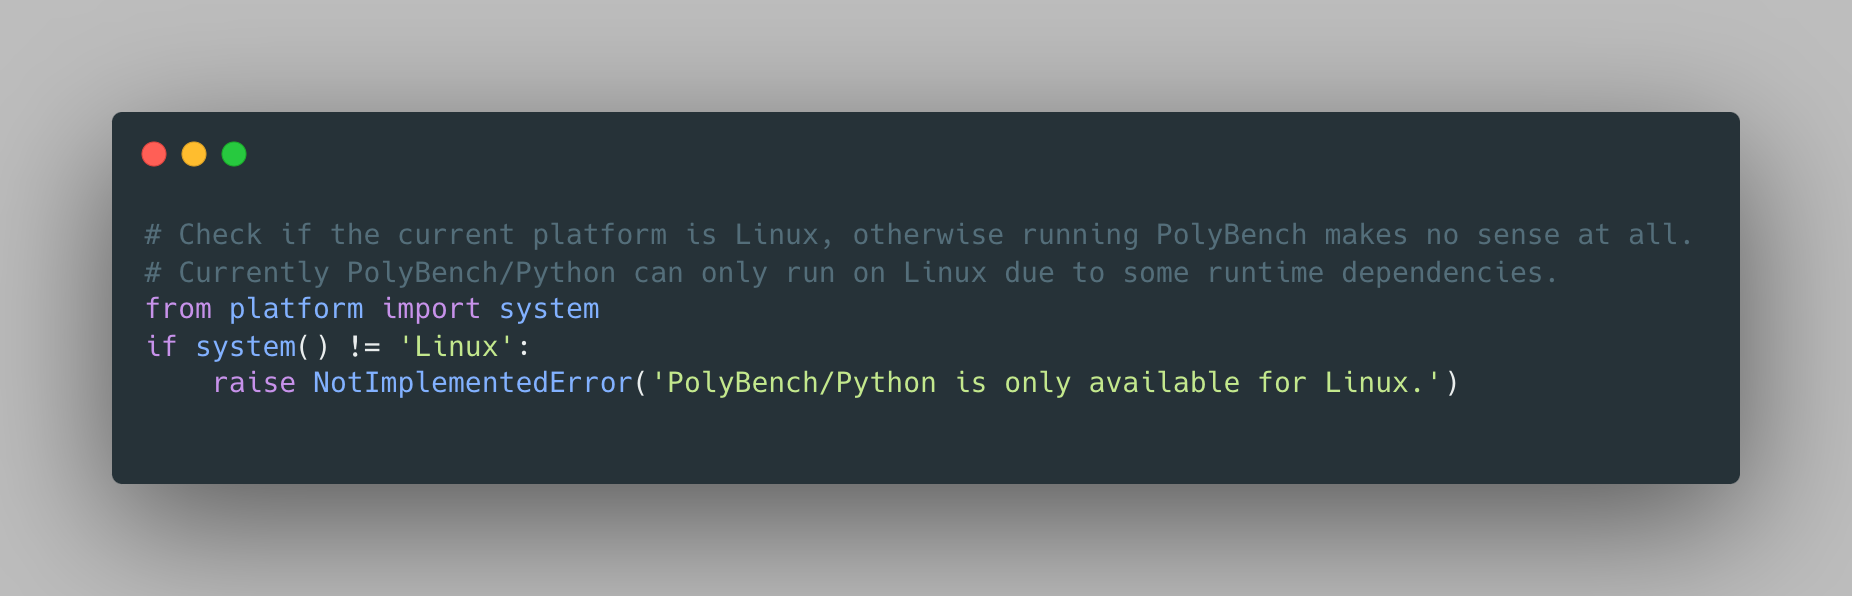
\includegraphics[scale=0.24]{polybench-python}
\caption{\footnotesize{Code snippet on PolyBench/Python compatibility}}
\captionsetup{aboveskip=0pt,font=it}
\end{figure}
\bigskip

There are 30 benchmarking tests in PolyBench/C. Its operation covers the majority of everyday computing tasks. PolyBench/C includes numerical computations extracted from various applications. This includes \textbf{linear algebra}, \textbf{image processing}, \textbf{physics simulation}, \textbf{dynamic programming}, \textbf{statistics} and so on. Each benchmark test consists of a single \textbf{C} program file along with its header \textbf{H} file. The user runs the benchmark file by first compiling it to a UNIX executable file with a C compiler such as \textbf{gcc} or \textbf{clang} \cite{exp44} \cite{exp45}. After that, they can then generate the program's output by running it in a terminal application and passing in the desired name of the output file. Users can also pass in extra configuration options to alter the compilation process as well as the desired output. For example, to display the program execution time or to change the size of the input dataset.

The source code of the project can be found here: \href{https://web.cse.ohio-state.edu/~pouchet.2/software/polybench/}{\color{blue}{The Polyhedral Benchmark Suite}}. Here is a list of all benchmark tests (Version 4.2.1) and their descriptions:

\newpage
\bigskip
\begin{table}[h!]
\centering
\begin{tabular}{||c c||} 
\hline
Name & Description \\ [1ex] 
\hline\hline
 & \\
2mm & 2 Matrix Multiplications (alpha * A * B * C + beta * D) \\ 
 & \\
3mm & 3 Matrix Multiplications ((A*B)*(C*D)) \\ 
 & \\
adi & Alternating Direction Implicit solver \\ 
 & \\
atax & Matrix Transpose and Vector Multiplication \\ 
 & \\
bicg & BiCG Sub Kernel of BiCGStab Linear Solver \\ 
 & \\
cholesky & Cholesky Decomposition \\ 
 & \\
correlation & Correlation Computation \\ 
 & \\
covariance & Covariance Computation \\ 
 & \\
deriche & Edge detection filter \\ 
 & \\
doitgen & Multi-resolution analysis kernel (MADNESS) \\ 
 & \\
durbin & Dynamic programming (2D) \\ 
 & \\
dynprog & Toeplitz system solver \\ 
 & \\
fdtd-2d & 2-D Finite Different Time Domain Kernel \\ 
 & \\
gemm & Matrix-multiply C=alpha.A.B+beta.C \\ 
 & \\
gemver & Vector Multiplication and Matrix Addition \\ 
 & \\
gesummv & Scalar, Vector and Matrix Multiplication \\
 & \\
gramschmidt & Gram-Schmidt decomposition \\ 
 & \\
head-3d & Heat equation over 3D data domain \\ 
 & \\
jacobi-1D & 1-D Jacobi stencil computation \\ 
 & \\
jacobi-2D & 2-D Jacobi stencil computation \\ [1ex]
\hline
\end{tabular}
\caption{PolyBench/C Benchmarks}
\label{table:time_complexity_2}
\end{table}

\begin{table}[h!]
\centering
\begin{tabular}{||c c||} 
\hline
Name & Description \\ [1ex] 
\hline\hline
 & \\
lu & LU decomposition \\ 
 & \\
ludcmp & LU decomposition followed by Forward Substitution \\ 
 & \\
mvt & Matrix Vector Product and Transpose \\ 
 & \\
nussinov & Dynamic programming algorithm for sequence alignment \\ 
 & \\
seidel & 2-D Seidel stencil computation \\ 
 & \\
symm & Symmetric matrix-multiply \\ 
 & \\
syr2k & Symmetric rank-2k update \\ 
 & \\
syrk & Symmetric rank-k update \\ 
 & \\
trisolv & Triangular solver \\ 
 & \\
trmm & Triangular matrix-multiply \\ [1ex]
\hline
\end{tabular}
\caption{PolyBench/C Benchmarks (continued)}
\label{table:time_complexity_2}
\end{table}

We continue our experiment by start utilising the PolyBench/C code. We designed a program that compiles and executes all \textbf{30} algorithms with \textbf{5} different data sizes: \textbf{mini}, \textbf{small}, \textbf{medium}, \textbf{large} and \textbf{extra large}.

The program will first construct a list of relevant paths of all benchmark files from the pre-set dictionary of \mintinline{python}{ALL_FILES}. After that, the program will create a temporary folder in the project root directory called \mintinline{Python}{compiled}. It will then compile all benchmarks into compiled UNIX executable binary files using the gcc compiler and store them in the \mintinline{Python}{compiled} folder. After its compilation, we will run the program with the 5 aforementioned dataset sizes for each benchmark. After running the binary executable files, we can output and log their runtimes. We do this by writing them in a text file with the naming convention (see below) and saving it persistently in a folder named \mintinline{python}{results}, which is also in the project root directory. Finally, after collecting all the results, we cleaned up the runtime environment by removing the \mintinline{Python}{compiled} folder.

\textbf{Result file naming convention:}
\newline
\mintinline{python}{output-file-<current date and time (Day-Month-Year-Hour-Minute-Second)>.txt}

The program source code is available publicly on GitHub.
\newline
The link can be found \href{https://github.com/richard875/Honours-PolyBench}{\color{blue}{here (GitHub: richard875/Honours-PolyBench)}}

After developing the PolyBench testing project, we are ready to integrate it with our testing frameworks. The PolyBench testing project was designed to be used as a "module". We achieve this by implementing and exposing a \mintinline{Python}{main} function that can be called externally and returns the runtime benchmark data.

We first integrate it with the Flask framework. We develop and configure the project so that it calls the \mintinline{python}{main} function on receiving a connection on a particular route, in this case, the index \mintinline{python}{/} route, then return and display the timing data on render.

We then integrate it with the Spin WebAssembly framework. We did essentially the same with the flask framework. We also point to the index route to execute the \mintinline{python}{main} function. However, this time the program failed to execute, and the benchmarks did not compile.

After conducting further research, we found that this is an expected behaviour for WebAssembly frameworks. As stated in the literature review section, one of the main benefits of WebAssembly is its security. WebAssembly applications execute in a sandboxed environment separated from the host environment and only expose limited APIs that were proven safe for developers to use \cite{exp46}. Therefore, in a WebAssembly environment, code such as \mintinline{Python}{os.path.isdir(RUNTIME_OUTPUT_FOLDER)} which checks if a directory exists or \mintinline{Python}{shutil.rmtree(RUNTIME_OUTPUT_FOLDER, ignore_errors=True)}, which deletes a directory folder along with all its contents will not work.

Therefore, we had to stop pursuing this experiment path and change our direction.

\bigskip
\section{Initial Dataset}

After the previous roadblock, we started to look for other benchmarking solutions. After further research, we decided that we would start the experiment with a custom collection of sorting algorithms. Some of the most popular sorting algorithms out there include \textbf{Bubble sort} \cite{exp47}, \textbf{Insertion sort} \cite{exp48} and \textbf{Quick sort} \cite{exp49}. Sorting algorithms are an excellent way to benchmark the runtime for individual web frameworks as they don't require any incoming or outgoing connections and thus, do not have any uncontrollable external factors. Also, unlike PolyBench, they do not need to be compiled into standalone files to run. Furthermore, sorting algorithms are also available in multiple languages (we will use Python in our case). As such, they can be run in almost any environment and platform.

During our experiment, we found that it is very difficult to come up with a set of "one-fits-all" number list input. For instance, some sorting algorithms in our collection take massively longer to complete than others.

We define our list input size (number of elements in the input list) as \(N\). We then set \(N = 1000\) and run the algorithm in the local environment. Faster sorting algorithms, such as \textbf{Quick sort} and \textbf{Merge sort}, took 0.002s and 0.004s to run respectively, while slower sorting algorithms, such as \textbf{Gnome sort} and \textbf{Brick sort}, took 0.123s and 11.171s respectively.

Here is a list of \textbf{18} sorting algorithms in our collection with their runtime boundary notation:

\bigskip
\begin{table}[h!]
\centering
\begin{tabular}{||c c c c||} 
\hline
Name & Best (Time) & Average (Time) & Worst (Time) \\ [1ex] 
\hline\hline
 & & & \\
Bitonic Sort & \(\Theta(log^2(n))\) & \(O(log^2(n))\) & \(\Omega(nlog^2(n))\) \\ 
 & & & \\
Bubble Sort & \(\Theta(n)\) & \(O(n^2)\) & \(\Omega(n^2)\) \\ 
 & & & \\
Brick/Odd-even Sort & \(\Theta(n)\) & \(O(n^2)\) & \(\Omega(n^2)\) \\ 
 & & & \\
Bucket Sort & \(\Theta(n)\) & \(O(n+\dfrac{n^2}{k}+k)\), \(k\) is number of buckets & \(\Omega(n^2)\) \\ 
 & & & \\
Cocktail Sort & \(\Theta(n)\) & \(O(n^2)\) & \(\Omega(n^2)\) \\ 
 & & & \\
Comb Sort & \(\Theta(nlog(n))\) & \(O(\dfrac{n^2}{2^p})\), \(p\) is number of increments & \(\Omega(n^2)\) \\ 
 & & & \\
Gnome Sort & \(\Theta(n)\) & \(O(n^2)\) & \(\Omega(n^2)\) \\ 
 & & & \\
Heap Sort & \(\Theta(nlog(n))\) & \(O(nlog(n))\) & \(\Omega(nlog(n))\) \\ 
 & & & \\
Insertion Sort & \(\Theta(n)\) & \(O(n^2)\) & \(\Omega(n^2)\) \\ [1ex]
\hline
\end{tabular}
\caption{Time complexity of sorting algorithms}
\label{table:time_complexity_1}
\end{table}

\begin{table}[h!]
\centering
\begin{tabular}{||c c c c||} 
\hline
Name & Best (Time) & Average (Time) & Worst (Time) \\ [1ex] 
\hline\hline
 & & & \\
Merge Sort & \(\Theta(nlog(n))\) & \(O(nlog(n))\) & \(\Omega(nlog(n))\) \\ 
 & & & \\
Pancake Sort & \(\Theta(n)\) & \(O(n^2)\) & \(\Omega(n^2)\) \\
 & & & \\
Pigeonhole Sort & \(\Theta(N+n)\) & \(O(N+n)\) & \(\Omega(N+n)\), \(N\) is key value range \\ 
 & & & \\
Quick Sort & \(\Theta(nlog(n))\) & \(O(nlog(n))\) & \(\Omega(n^2)\) \\ 
 & & & \\
Radix Sort & \(\Theta(nk)\) & \(O(nk)\) & \(\Omega(nk)\), \(k\) is key length \\
 & & & \\
Selection Sort & \(\Theta(n^2)\) & \(O(n^2)\) & \(\Omega(n^2)\) \\ 
 & & & \\
Shell Sort & \(\Theta(nlog(n))\) & depends & \(\Omega(n^2)\) \\ 
 & & & \\
Smooth Sort & \(\Theta(n)\) & \(O(nlog(n))\) & \(\Omega(nlog(n))\) \\ 
 & & & \\
Strand Sort & \(\Theta(n)\) & \(O(n^2)\) & \(\Omega(n^2)\) \\ [1ex]
\hline
\end{tabular}
\caption{Time complexity of sorting algorithms (continued)}
\label{table:time_complexity_2}
\end{table}
\bigskip

\bigskip
\section{First Stage: Sorting Algorithm Development}

We are now ready to start experimenting. The first stage of our experiment is to design and develop the algorithm collection. In this step, we gathered all \textbf{18} different algorithms of our choice. We collected the algorithm code from websites such as \href{https://www.geeksforgeeks.org/}{\color{blue}{geeksforgeeks.org}} and \href{https://www.programiz.com/}{\color{blue}{programiz.com}}. After that, we performed local tests on each algorithm function to ensure that they were able to produce their desired outcome.

Each algorithm is essentially its own file. As stated above, the algorithm does not produce any outgoing traffic connections, and it also doesn't have any import modules, as we would like to keep uncontrolled factors to a minimum. Therefore, they are standalone codes that can be executed on any platform. We also implemented \mintinline{python}{if __name__ == "__main__" :} module code in the algorithm files to prevent the code from being executed upon importation.

After all the algorithms were packaged and tested, we grouped all files into a folder to be used as a module. And then, we created our testing files to run and measure the time for each algorithm.

In our testing file, we imported all the algorithms from the above folder to be used during measurement. Furthermore, we will be using the Python \mintinline{Python}{time} and \mintinline{Python}{random} modules. At the beginning of the testing script, we constructed the arrays to be performed on. We do this by generating a number between 0 and \(N\), where \(N\) is either a fixed parameter defined within the script or passed in during runtime. Then, for each array, we run this process \(L\) times, where \(L\) is the length of the array. In this case, \(N = L\).

As stated above, different sorting algorithms significantly differ in performance and runtime. Therefore, it is difficult at best and almost impossible at worst to come up with a "one-for-all" array length to test the benchmarks for all sorting algorithms. This can be observed in Bingmann's 2013 article "The Sound of Sorting" \cite{exp50}. In the article and the subsequent video \cite{exp51}, different algorithms are given different input lengths to achieve a similar runtime. For example, \textbf{selection sort} and \textbf{quick sort} both completed sorting in similar timeframes. However, selection sort only had an array input size of 130, yet quick sort had an array input size of 1440. The GitHub repository for the project can be found here \cite{exp52}. Our solution to this is to perform local tests with different input sizes to get a rough estimate of the time complexity for each algorithm. In the experiment, we will run each algorithm \textbf{5} times with \textbf{3} input array sizes - \mintinline{Python}{small}, \mintinline{python}{medium} and \mintinline{python}{large}. In our local tests, we set our \mintinline{python}{small} input size to be run within around \textbf{2} seconds, \mintinline{Python}{medium} input size to be run within around \textbf{5} seconds and \mintinline{Python}{large} input size to be run within around \textbf{10} seconds. This is the performance benchmark we observed when running locally. However, we are fully expecting a drop in performance for both frameworks when running remotely in production due to various overheads as well as the increased physical distance between the client and the server.

Here is a list of detailed array input sizes \(N\) for each sorting algorithm:
\begin{table}[h!]
\centering
\begin{tabular}{||c c c c||} 
\hline
Name & Small & Medium & Large \\ [1ex] 
\hline\hline
 & & & \\
Bitonic Sort & 100000 & 200000 & 300000 \\ 
 & & & \\
Bubble Sort & 5000 & 7000 & 10000 \\ 
 & & & \\
Brick/Odd-even Sort & 600 & 800 & 1000 \\ 
 & & & \\
Bucket Sort & 35000 & 55000 & 70000 \\ 
 & & & \\
Cocktail Sort & 4000000 & 10000000 & 17000000 \\ 
 & & & \\
Comb Sort & 250000 & 550000 & 850000 \\ 
 & & & \\
Gnome Sort & 4000 & 6500 & 9000 \\ [1ex]
\hline
\end{tabular}
\caption{Array input sizes for sorting algorithms}
\label{table:time_complexity_1}
\end{table}

\begin{table}[h!]
\centering
\begin{tabular}{||c c c c||} 
\hline
Name & Small & Medium & Large \\ [1ex] 
\hline\hline
 & & & \\
Heap Sort & 200000 & 500000 & 900000 \\ 
 & & & \\
Insertion Sort & 6000 & 10000 & 14000 \\ 
 & & & \\
Merge Sort & 300000 & 700000 & 1400000 \\
 & & & \\
Pancake Sort & 4500 & 7000 & 10000 \\
 & & & \\
Pigeonhole Sort & 4000000 & 11000000 & 20000000 \\ 
 & & & \\
Quick Sort & 550000 & 1250000 & 2500000 \\ 
 & & & \\
Radix Sort & 450000 & 980000 & 1500000 \\
 & & & \\
Selection Sort & 6000 & 9500 & 14000 \\ 
 & & & \\
Shell Sort & 190000 & 400000 & 700000 \\ 
 & & & \\
Smooth Sort & 85000 & 200000 & 400000 \\ 
 & & & \\
Strand Sort & 20000 & 30000 & 35000 \\ [1ex]
\hline
\end{tabular}
\caption{Array input sizes for sorting algorithms (continued)}
\label{table:time_complexity_2}
\end{table}
\bigskip

\bigskip
\section{Framework Deployment}

Amazon Web Service (AWS) provides an excellent Paas platform for us to deploy both applications. We used services including \textbf{Amazon ec2}, \textbf{Amazon Elastic Container Registry (ECR)} and \textbf{Amazon Elastic Container Service (ECS)} \cite{exp53} \cite{exp54}.

We containerised both applications into Docker containers. We do this by adding a \mintinline{Python}{Dockerfile} file in the root of our project. Both applications use Ubuntu as the Docker container base image \cite{exp55}.

For our Flask application, we install \mintinline{Python}{python3-pip}, as well as \mintinline{python}{Flask}. We then copy all files into the Docker container and finally start the application in the Docker container by running the\newline\mintinline{Python}{python3 -m flask run --host=0.0.0.0} command. We use \mintinline{Python}{--host=0.0.0.0} to host the application on the server's public IPv4 address to be accessible on port 5000.

For our Spin application, we needed to install the spin runtime provided by Fermyon from a bash script \cite{exp56}. However, before that, we first need to install all dependencies needed to run the script. These are: \mintinline{python}{curl}, \mintinline{python}{build-essential}, \mintinline{python}{libssl-dev} and \mintinline{python}{pkg-config}. After that, we install the spin runtime binary by running the \mintinline{Python}{install.sh} script. Finally, we start the application by running the \newline\mintinline{Python}{./docker/Spin up --listen 0.0.0.0:3000} command.

We upload our applications to Amazon Web Service, both on ec2 instances. However, with our Spin application, we will be using the Amazon CloudFront service to distribute the application to edge machines around the world \cite{exp57}. Amazon CloudFront has edge locations worldwide, including major cities such as \textbf{London}, \textbf{New York}, \textbf{Sydney}, \textbf{Shanghai} and \textbf{Hong Kong}.

\bigskip
\section{Second Stage: Dijkstra, Floyd, Kruskal and Prim}

We conducted the first stage of our experiment. And we listed the detailed data in the \textbf{Results} section. To our surprise, and in contradiction to the initial hypothesis, which suggested that the Spin WebAssembly framework would perform better, we observed the opposite. On average, across all tests and benchmarks, Flask outperformed Spin by \textbf{140\%}.

Based on the result from the first stage of the experiment, we decided to continue and expand on benchmarking our frameworks. By this stage of the experiment, we are able to recognise that Flask performs better than Spin. But we want to discover if there are any differences between the performance gap for both frameworks running different kinds of algorithms (non-sorting algorithms). Therefore, we further introduced 4 algorithms: \textbf{Dijkstra's algorithm}, \textbf{Floyd–Warshall algorithm}, \textbf{Kruskal's algorithm} and \textbf{Prim's algorithm}. Similar to sorting, we will run each algorithm \textbf{5} times, inputting \textbf{3} datasets with different sizes.

\bigskip
\subsection{Dijkstra's Algorithm}

In practice, we use Dijkstra's Algorithm to find the shortest distance between two points on a map. However, we usually represent this by finding the shortest path between two vertices in a graph \cite{exp58}. In our benchmarking test, we set \(V\) to the number of vertices on a side with the total number of vertices being \(V^2\). Furthermore, each vertex is connected by an edge with a weight (distance) randomly generated between 0 and 20.

We run the algorithm on every pair of vertices, totalling to \(V(V-1)/2\) pairs. As a result, the average runtime complexity is \(O(E+V\cdot\ Log(V))\) where \(E\) is the number of edges in the graph and \(V\) is the number of vertices in the graph. The size of the input datasets (number of edges) is \textbf{2500}, \textbf{4000} and \textbf{5800}, respectively. Thus, the total runtime for our Dijkstra's Algorithm benchmarking test is:

\[ O(V(V-1)/2 \cdot (E+V\cdot\ Log(V))\ where\ V \in \{2500, 4000, 5800\}, V = E \]

\bigskip
\subsection{Floyd–Warshall Algorithm}

The Floyd–Warshall Algorithm, also called Floyd's Algorithm, is a non-greedy shortest path algorithm \cite{exp59}. However, unlike Dijkstra's Algorithm, Floyd–Warshall Algorithm does not work on graphs with negative cycles. In our benchmarking test, we set \(V\) to the number of vertices on a side with the total number of vertices being \(V^2\). We then set \(E\) to be the number of all edges in the graph where \(V = E\). Each edge has a 50\% chance of having an infinite weight. When this occurs, we consider the pair of vertices not connected. For connected edges, each has a weight distance randomly generated between 0 and 20.

We then run the algorithm on every pair of vertices, totalling to \(V(V-1)/2\) pairs. The average runtime complexity is \(O(V^3)\), where \(V\) is the number of vertices in the graph. The size of the input datasets (number of edges) is \textbf{180}, \textbf{250} and \textbf{310}, respectively. Thus, the total runtime for our Floyd's Algorithm benchmarking test is:

\[ O(V(V-1)/2 \cdot V^3) \]
\[ =O(V^4(V-1)/2)\ where\ V \in \{180, 250, 310\}  \]

\textbf{Note:} We observed that Floyd's Algorithm has a greater runtime complexity than Dijkstra's Algorithm. Thus, in order to keep the runtime similar, we reduced the input sizes for Floyd's Algorithm.

\bigskip
\subsection{Kruskal's Algorithm}

Kruskal's Algorithm is a greedy, minimum-spanning tree algorithm \cite{exp60}. A \textbf{minimum spanning tree} returns a list of edges where the sum of their weights is as small as possible \cite{exp61}.

\begin{figure}[hp]
\centering
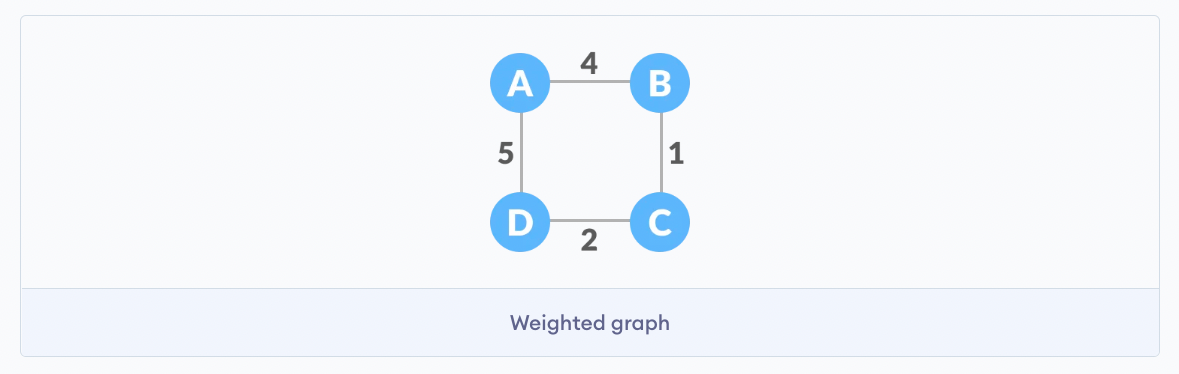
\includegraphics[scale=0.4]{minimum-spanning-tree-1}
\caption{\footnotesize{A Weighted Undirected Graph \cite{expa1}}}
\captionsetup{aboveskip=0pt,font=it}
\end{figure}
\bigskip

\begin{figure}[hp]
\centering
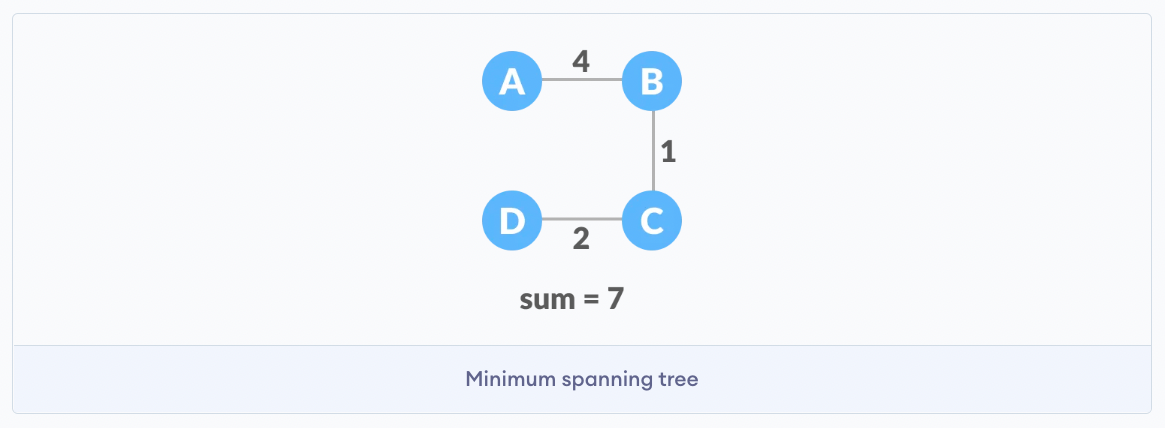
\includegraphics[scale=0.4]{minimum-spanning-tree-2}
\caption{\footnotesize{Minimum Spanning Tree for the above Graph, in this case, 7 (4 + 1 + 2) \cite{expa1}}}
\captionsetup{aboveskip=0pt,font=it}
\end{figure}
\bigskip

In our testing script, we again set \(V\) to the number of vertices on a side with the total number of vertices being \(V^2\). Furthermore, we define \(E\) as edge, where \(E = V - 1\). Each \(E\) connects \(V[i]\) with \(V[i+1]\), where \(i\) is the index of \(E\).

We then run the algorithm on the graph and measure its runtime. The algorithm finds and traverses through the minimum spanning tree of our graph. The average runtime complexity is \(O(E\cdot\ Log(E))\), where \(E\) is the total number of edges in the graph. The size of the input datasets (number of edges) is \textbf{400000}, \textbf{1000000} and \textbf{2100000}, respectively. Thus, the total runtime for our Kruskal's Algorithm benchmarking test is:

\[ O(E\cdot\ Log(E))\ where\ E = V - 1, V \in \{400000, 1000000, 2100000\} \]
\[ =O(E\cdot\ Log(E))\ where\ E \in \{399999, 999999, 2099999\} \]

\bigskip
\subsection{Prim's Algorithm}

Finally, we benchmark Prim's Algorithm. Just like Kruskal's Algorithm, Prim's Algorithm is a greedy, minimum-spanning tree algorithm \cite{exp62}. However, unlike Kruskal's Algorithm, Prim's Algorithm selects the root vertex upon execution and gradually expands outwards until it has traversed the whole graph \cite{exp63}. In our benchmarking test, we set \(V\) to be the number of vertices on a side, with the total number of vertices being \(V^2\). After that, just like Floyd's Algorithm, we set \(E\) to be the number of all edges in the graph where \(V = E\). Each edge has a 50\% chance of having a zero (0) weight. When this occurs, we consider the pair of vertices not connected. For connected edges, each has a weight distance randomly generated between 1 and 99.

We then run the algorithm on the graph and measure its runtime. Prim's Algorithm finds and traverses through the minimum spanning tree of our graph. Its average runtime complexity is \(O(E\cdot\ Log(V))\) where \(V\) is the number of vertices in the graph and \(E\) is the number of edges in the graph. The size of the input datasets (number of edges) is \textbf{400}, \textbf{550} and \textbf{680}, respectively. Thus, the total runtime for our Prim's Algorithm benchmarking test is:

\[ O(E\cdot\ Log(V))\ where\ E, V \in \{400, 550, 680\} \]

\bigskip
\section{The Next Episode}

After conducting both stages of our experiment, we present our findings in the \textbf{results} section. Also in the next section, we will analyse our results and present exciting and unexpected discoveries.